\section{Memory Transfer Optimization}
\label{sec:transfer}
\subsection{Pinned Memory}
\label{pinned}
One of the most important aspects of optimization is the memory transfer between host and device.\\
% todo check
Unfortunely, as we have seen in table \ref{tab:pci_comp}, the link bandwidth between host and device is by up to a order lower than bandwidth to device memory.\\
Memory transfer without modifications uses pageable memory to copy data from host to device and vice versa.\\
Using pageable memory is problematic, because as soon as the device requests access to host memory (for example for memory copies)
the host has to check whether the data resides in physical memory or if it has been swapped out.\\
This results in a non-trivial CPU load and therefore lowers the bandwidth.\\
To avoid this, it is possible to request so-called page-locked, or \emph{pinned memory} which is not eligible to swapping.\\
Page-locked memory results generally in a much higher bandwidth, although this difference is influenced by the CPU where a system
with a stronger CPU performs better than a system with a weaker processor on pageable memory but in all instances slower than pinned memory.\\
Without the involvement of the processor, the OS has to fulfil the demand that page-locked memory is \textbf{always} backed by physical memory,
so the device can setup a direct memory access (DMA).\\\\
Thus, one of the simpliest yet most effective ways to improve memory transfer bandwidth results into higher bandwidth and lower CPU load for the host.\\\\
% todo: write about how awesome i am
Using consumer-grade hardware the following data has been determined to display the differences of the two memory in Figure \ref{fig:bandwidth}.\\
% which has 
\begin{figure*}[ht]
    \centering
%    \includegraphics[scale=0.5,natwidth=1200,natheight=800]{media/bandwidth_pageable_vs_pinned_both3.png}
    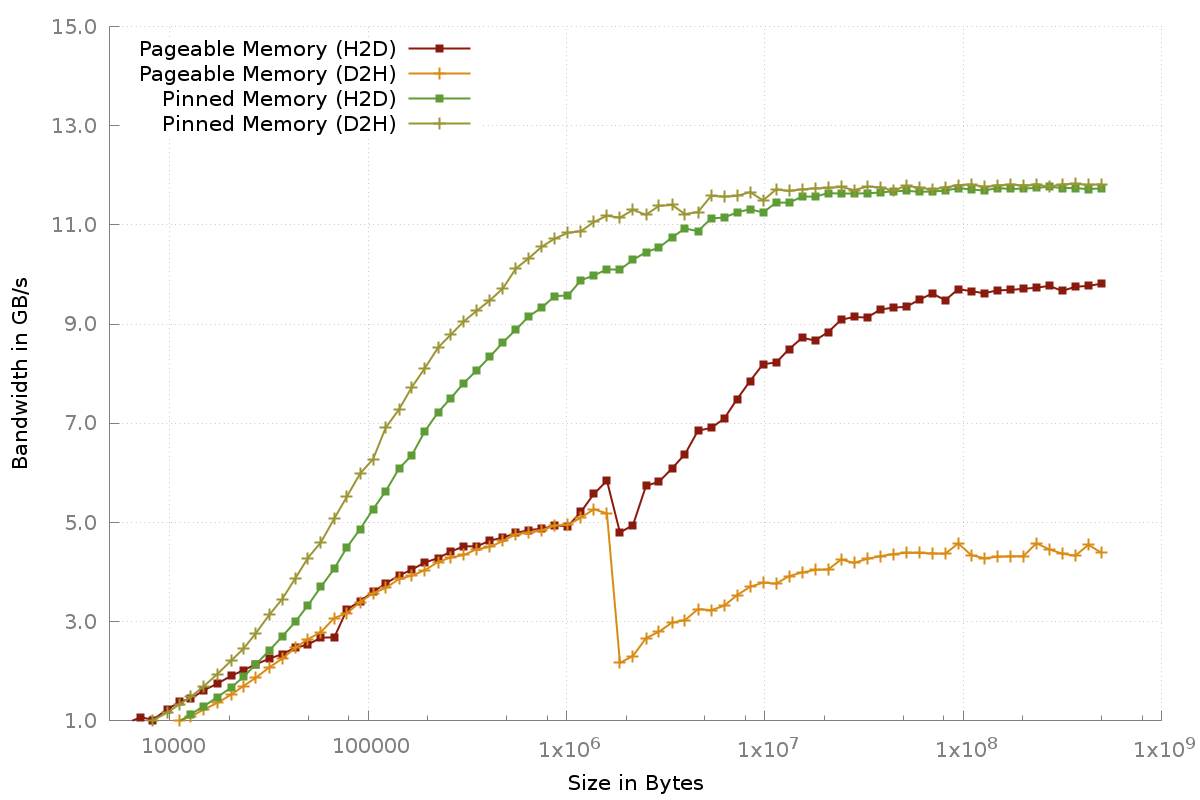
\includegraphics[scale=0.35,natwidth=1200,natheight=800]{media/bandwidth_both.png}
    \caption{Comparison of Pinned to Pageable Memory}
    \caption*{System: Linux 64-bit with GTX 750 1GB CC 5.0, CUDA 7.5, Intel(R) i5-4670 @ 3.40 GHz}
    \caption*{Source code: \href{https://github.com/spotlight0xff/cuda\_paper/code/bandwidth}{On Github}}
    \label{fig:bandwidth}
\end{figure*}
% discuss results
These results have been recorded by allocating memory sizes linearly distributed in a logarithmic space up to 512 MB with sizes aligned to at least 512 bytes, using respectively pageable and pinned memory.\\
To reduce the influence of statistical errors on the data, the recordings have been averaged over 200 measurements.\\
The figure shows clearly the significant speed-up provided by pinned memory, especially in the case of device to host transfer
where pinned memory shows no notable difference between the transfer direction.\\
%Even though the overall results may be expected, the displayed disparity between the pageable memory transfers can be surprising. (explanation...?)\\\\

While host memory is page-locked, it can't be used by the operating systems memory management,
which may result in degraded systems performance due to insufficient memory available.\\
Another notable pitfall of pinned memory is the increased allocation time as we will see in the next paragraph.\\
\subsubsection{Registering Host Memory}
In some cases it is desirable to not allocate pinned memory, but to flag already allocated host memory as pinned memory.\\
This is especially interesting for applications with an addon framework where addons can provide host memory.
The framework provider could then registers it as page-locked using \emph{cudaHostRegister()}, operates on the accelerated memory and later unregister it with \emph{cudaHostUnregister()}.\\
\begin{table}[ht]
\centering
\begin{tabular}{SSS}
    \textbf{Size} & \textbf{Allocation} & \textbf{Registration}\\
\hline
\textbf{\SI{512}{\byte}} & \SI{0.30}{\milli\second}  & \SI{0.08}{\milli\second}\\
\textbf{\SI{1}{\mebi\byte}}      & \SI{0.28}{\milli\second}  & \SI{0.23}{\milli\second}\\
\textbf{\SI{10}{\mebi\byte}}     & \SI{2.01}{\milli\second}  & \SI{0.95}{\milli\second}\\
\textbf{\SI{200}{\mebi\byte}}    & \SI{37.92}{\milli\second} & \SI{17.83}{\milli\second}\\
\textbf{\SI{500}{\mebi\byte}}    & \SI{94.30}{\milli\second} & \SI{44.11}{\milli\second}\\
\hline
\end{tabular}
\caption{Allocation times of pinned memory versus registering host memory}
\caption*{System: GTX 750 1GB CC 5.0 with CUDA 7.5}
\caption*{Source code: \href{https://github.com/spotlight0xff/cuda\_paper/code/alloc/}{on GitHub}}
\label{tab:host_reg_pinned}
\end{table}
The allocation times shown in table \ref{tab:host_reg_pinned} are roughly doubling the registration times for memory sizes of more than a few megabytes, which is to be expected
as we don't have to explicit allocate the memory and rather just mark it pinned.\\
\subsubsection{Portable Pinned Memory}
Pinned Memory can be allocated or registered portable when it is required to be accessed by multiple CUDA units,
because an allocation made by one GPU is by default only accessible to the allocator.\\
% todo
To use portable pinned memory you can set the $flags$ argument of \emph{cudaHostAlloc} or \emph{cudaHostRegister} to \emph{cudaHostAllocPortable} or \emph{cudaHostRegisterPortable}, respectively.
%todo: need \cite
With UVA in effect, pinned memory is per default marked portable.
% same as zero-copy!
%\subsubsection{Mapped Pinned Memory}
%To map pinned memory directly into the GPU address space, enabling the developer to access 
%in CUDA 2.2, it is possible to map pinned memory directly into the CUDA address space, which enables the developer to write directly to host memory.\\
%This eliminates the need for device memory allocation, especially in a situation where data has to be only read or written once, it is preferable to use mapped memory instead of memory copies.\\
%Using mapped pinned memory it is important to align the data properly to have its access coalesced as described in ~\ref{global_access}.
%With UVA in effect, CPU and GPU share the same address space and therefore the same address can be used so there is no need to update both allocation tables.
\subsection{Zero-Copy}
\label{zerocopy}
%\cite{doc_cuda22_pinnedmem}
%\cite{wrox_zero_copy}
Mapped pinned memory, or \emph{zero-copy} memory, is a feature introduced in CUDA 2.2\cite{doc_cuda22_pinnedmem} to allow direct access to host memory without explicit memory copies.\\
Zero-copy memory can be allocated similar to portable pinned memory by providing \emph{cudaHostAllocMapped} or \emph{cudaHostRegisterMapped} to a call of either \emph{cudaHostAlloc} or \emph{cudaHostRegister}.
Additionally it is required to call \emph{cudaSetDeviceFlags(cudaDeviceMapHost)} to enable zero-copy.\\
Similiarly to Unified Memory, it can be used to avoid explicit data transfer by transparently copying the pinned memory to device memory only when needed.\\
This is particularly useful if the GPU lacks sufficient device memory even though this adds latency to the application.\\
% beneficial
In the case of an integrated GPU zero-copy memory is always beneficial, because the host and the device share the same physical memory. Therefore it is unnecessary to perform additional memory copies.\\
% possibility
Another interesting use of mapped pinned memory is the possibility to possible to enable overlapping memory transfer with kernel execution.\\
Overlapping is normally performed using multiple streams where only parts of the memory is copied at once as outlined in \ref{streams}.\\
%% data are only!!
CUDA simplifies this process with zero-copy, where the data transfer is done transparently similar to the Unified Memory concept ( see \ref{unifiedmemory} ) where data is only transferred when needed.
This technique is only possible and beneficial due to DMA. Without it, a host thread would have to receive and perform the memory transfers accordingly, resulting in higher system load and lower throughput.\\
Additionally to overlapping, zero-copy can also be used to access complex structures without performing expensive deep copies, again similar to Unified Memory.\\
